\documentclass{article}
\linespread{1.3}
\usepackage[margin=50pt]{geometry}
\usepackage{amsmath, amsthm, amssymb, amsthm, tikz, fancyhdr, graphicx}
\pagestyle{fancy}
\renewcommand{\headrulewidth}{0pt}
\newcommand{\changefont}{\fontsize{15}{15}\selectfont}

\fancypagestyle{firstpageheader}
{
  \fancyhead[R]{\changefont Michael Huang \\ CFRM 420 \\ Homework 8}
}

\begin{document}

\thispagestyle{firstpageheader}

\section*{1.}
{\Large 
\subsection*{(a)}

For the ARMA process given by (1), $X_t + 0.5X_{t-1} = \varepsilon_t + \varepsilon_{t-1} - \varepsilon_{t-2}$, or $\phi(z) = 1 + 0.5z$ we implement in this R. We have $\phi_1 = 0.5$, and solving gives us the root $z = -2$, which is not a zero within the unit circle on the complex plane, so there exists a causal stationary solution to this ARMA process.

\subsection*{(b)}

For the ARMA process given by (2), $X_t - \frac{3}{2}X_{t-1} + \frac{1}{2}X_{t-2}= \varepsilon_t + \varepsilon_{t-1} - \varepsilon_{t-3}$, we implement in this R. We have that $\phi_1 = -\frac{3}{2}, \phi_2 = \frac{1}{2}$; solving this gives us the roots $z = 1, 2$ in the complex plane, so none of the zeros are within the unit circle on the complex plane, so there does exist a causal stationary solution to this ARMA process. \\ \\
For the ARMA process given by (3), $X_t - 5X_{t-1} + 8X_{t-2} - 2X_{t-5}= 2\varepsilon_t$, we implement in this R. We have that $\phi_1 = -5, \phi_2 = 8, \phi_5 = -2$; solving this gives us the zeros $z = 0.3575712, 0.3575712, 1.7073595, 1.3415130, and 1.7073595$ in the complex plane, which does have some causal stationary solutions since some zeros are not within the unit circle on the complex plane, but others are, and thus are not causal stationary solutions.
\newpage

}

\section*{2.}
{\Large 
\subsection*{(a)}

We assume values of $h$ above max$\{p, q\}$. We take the covariance of $X_{t-h}$ and the right-hand side of (1) to get a covariance of 0. We then take the covariance of $X_{t-h}$ and the left-hand side of (1) to get $\gamma(h) + 0.5\gamma(h-1)$. We equate these two covariances to get \\
$\gamma(h) + 0.5\gamma(h-1) = 0.$ \\
which is exactly what we sought to find.

\subsection*{(b)}

We continue for the value of $h=0$. We take the covariance of $X_{t-h}$ and the right-hand side of (1) in this case to get \\ $\text{Cov}(X_t, \varepsilon_t + \varepsilon_{t-1} - \varepsilon_{t-2})$ \\ 
$= \text{Cov}(\varepsilon_t + \varepsilon_{t-1} - \varepsilon_{t-2} - 0.5X_{t-1}, \varepsilon_t + \varepsilon_{t-1} - \varepsilon_{t-2})$ \\ 
$= -0.5\text{Cov}(\varepsilon_{t-1} + \varepsilon_{t-2} - \varepsilon_{t-3} - 0.5X_{t-2}, \varepsilon_t + \varepsilon_{t-1} - \varepsilon_{t-2}) + \sigma^2 + \sigma^2 + \sigma^2$ \\ 
$= 0.25\text{Cov}(\varepsilon_{t-2} + \varepsilon_{t-3} - \varepsilon_{t-4} - 0.5X_{t-3}, \varepsilon_t + \varepsilon_{t-1} - \varepsilon_{t-2}) + 3 + \sigma^2 - \sigma^2$ \\ 
$= -0.25\sigma^2 + 3$ \\ 
$= -0.25 + 3$ \\
$= 2.75$. \\
We then take the covariance of $X_{t-h}$ and the left-hand side of (1) to get $\gamma(h) + 0.5\gamma(h-1)$ yet again. We equate these expressions to get \\
$\gamma(h) + 0.5\gamma(h-1) = 2.75.$ \\
which is exactly what we sought to find.

\subsection*{(c)}

We continue for the value of $h=1$. We take the covariance of $X_{t-h}$ and the right-hand side of (1) in this case to get \\ $\text{Cov}(X_{t-1}, \varepsilon_t + \varepsilon_{t-1} - \varepsilon_{t-2})$ \\ 
$= \text{Cov}(X_{t-1}, \varepsilon_{t-1})$ \\ 
$= \text{Cov}(\varepsilon_{t-1} + \varepsilon_{t-2} - \varepsilon_{t-3} - 0.5X_{t-2}, \varepsilon_{t-1})$ \\
$= \text{Cov}(\varepsilon_{t-1} + \varepsilon_{t-2} - \varepsilon_{t-3} - 0.5X_{t-2}, \varepsilon_{t} + \varepsilon_{t-1} - \varepsilon_{t-2})$ \\
$= 0.5\text{Cov}(X_{t-2}, \varepsilon_{t-2}) + \sigma^2 - \sigma^2$ \\
$= 0.5\text{Cov}(\varepsilon_{t-2} + \varepsilon_{t-3} - \varepsilon_{t-4} - 0.5X_{t-3}, \varepsilon_{t-2})$ \\
$= 0.5\sigma^2$ \\
$= 0.5$. \\
We then take the covariance of $X_{t-h}$ and the left-hand side of (1) to get $\gamma(h) + 0.5\gamma(h-1)$ yet again. We equate these expressions to get \\
$\gamma(h) + 0.5\gamma(h-1) = 0.5.$ \\
which is exactly what we sought to find. \\ \\
We continue for the value of $h=2$. We take the covariance of $X_{t-h}$ and the right-hand side of (1) in this case to get \\ $\text{Cov}(X_{t-2}, \varepsilon_t + \varepsilon_{t-1} - \varepsilon_{t-2})$ \\ 
$= \text{Cov}(X_{t-2}, -\varepsilon_{t-2})$ \\ 
$= -\text{Cov}(\varepsilon_{t-2} + \varepsilon_{t-3} - \varepsilon_{t-4} - 0.5X_{t-3}, \varepsilon_{t-2})$ \\
$= -\sigma^2$ \\
$= -1$. \\
We then take the covariance of $X_{t-h}$ and the left-hand side of (1) to get $\gamma(h) + 0.5\gamma(h-1)$ yet again. We equate these expressions to get \\
$\gamma(h) + 0.5\gamma(h-1) = -1.$ \\
which is exactly what we sought to find. \\ \\
We put all of these Yule-Walker equations together into a system of linear equations in R and solve. We have $\textbf{c} = [2.75, 0.5, -1]$ and $A = \begin{bmatrix}
  1 & 0.5 & 0 \\
  0.5 & 1 & 0 \\
  0 & 0.5 & 1
  \end{bmatrix}$ \\ \\
Solving in R, we can verify that our result $\gamma$ is indeed $[3.3333333, -1.1666667, -0.4166667]$, which corresponds accordingly to $\gamma(0), \gamma(1), \gamma(2)$.

\subsection*{(d)}

We implement this in R, using the fact that $\rho(h) = \gamma(h) / \gamma(0)$ and substituting as necessary using equations 4-6 and the equation in part (a): \\
$\rho(0) = 1$ \\
$\rho(1) = -0.35$ \\
$\rho(2) = -0.125$ \\
$\rho(3) = 0.0625$ \\
$\rho(4) = -0.03125$ \\
$\rho(5) = 0.015625$ \\
% TODO: this is wrong
Using the ARMAacf function in R, we also verify these results.
\newpage

}

\section*{3.}
{\Large 

\subsection*{(a)}

We implement this in R: \\ 
\begin{figure}[h!]
  \centering
  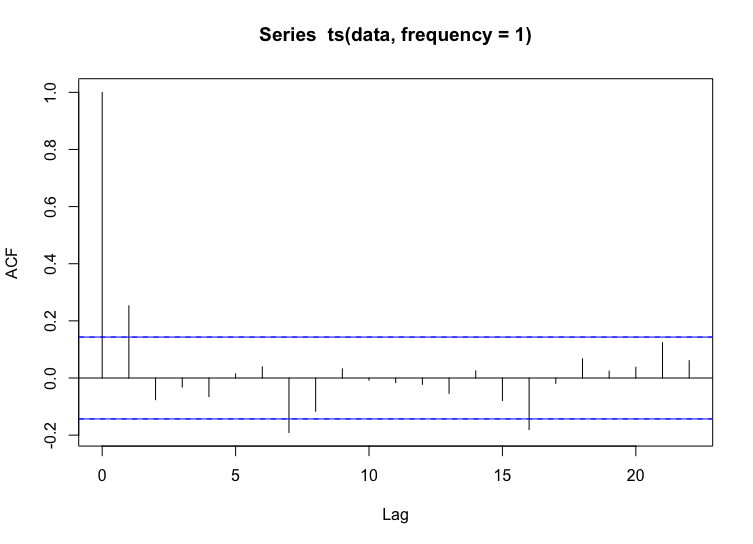
\includegraphics[width=500pt]{hw8_3a.png}
\end{figure}

\subsection*{(b)}

In regards to the hypothesis test at a 5\% significance level for $\rho(1) = 0$, we see that the value at $\rho(1)$ is well above the confidence intervals, so we successfully rejected the null hypothesis and find that $\rho(1) \neq 0$.

\subsection*{(c)}

Looking at the graphed sample autocorrelation function at the other lag values, we see that the null hyopethesis of zero autocorrelation is rejected at 2 lags. We would expect to see that the null hypothesis of zero autocorrelation would never be rejected outside the at a 5\% significance level if the data were independent white noise, since for independent white noise, $\hat{\rho}(h)$ should lie within the band; in the same vein, it is reasonable to assume the data follows MA(1) process since $\hat{\rho}(h)$ lies within the band for most $|h| > 1$, since for an MA(1) process, $\rho(h) = 0$ for all $|h| > 1$.
% TODO: check this reasoning for guessing how many times?

}

\end{document}